% Drawing 147/04-5 -- folder 147, batch 04, archive page 73 (PDF page 74).
% Transcription: schéma raturé : un graphe à deux sommets marqués $I' \setminus \{a'\}$ et $I''$, entouré d'un contour en forme de cloche ; en dessous, un segment dont l'extrémité gauche porte un symbole surchargé
% Kind: struck schema: graph in a bell-shaped contour. Method 2 (schematic redraw from the facsimile). Status: partial.
% Notes: Crossed out on the page: a bell-shaped contour round a graph whose two vertices are labelled I' \ {a'} and I''; below it a segment whose left end carries an overinked symbol (left out). The cross strokes are drawn grey (struck); the course of the contour is approximate; the two vertices themselves are not distinguishable from the strokes and are placed at their labels.
% Coordinates: 1 unit = 1 mm = 1/100 of the crop width (bbox in page fractions: [0.388, 0.619, 0.622, 0.723]).
% Redrawn by Claude (claude-opus-5-5), issue #73, 2026-11-07; not checked by a human; not compiled (no TeX in the session).
% Rights: reproduces part of the work -- behind RENDER_TRANSCRIPTS, never published by itself.
\documentclass[tikz,border=3pt]{standalone}
\usepackage{amsmath,amssymb}
\usetikzlibrary{patterns,arrows.meta}
\tikzset{pencil/.style={black!45}, struck/.style={black!35}, mark/.style={circle,draw,inner sep=1.3pt}, pt/.style={circle,fill,inner sep=0.9pt}, opt/.style={circle,draw,fill=white,inner sep=1.1pt}}
\begin{document}
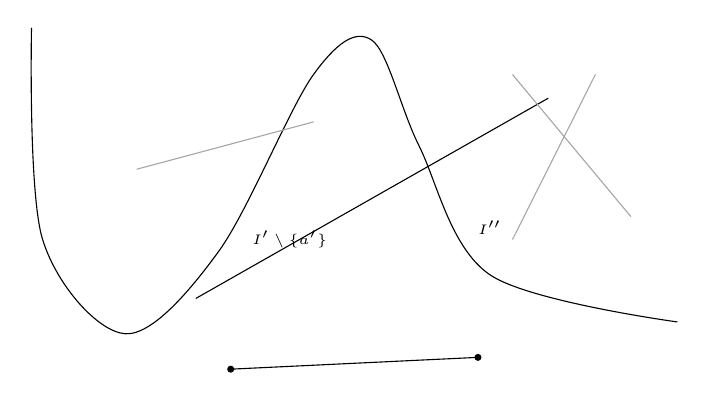
\begin{tikzpicture}[x=1mm,y=1mm,line cap=round,line join=round,font=\scriptsize]
\draw plot[smooth, tension=0.55] coordinates {(9,-6) (10.4,-32.8) (20.9,-44.8) (32.8,-34.3) (44.8,-11.9) (52.2,-7.5) (58.2,-20.9) (67.2,-37.3) (91,-43.3)};
\draw (29.9,-40.3) -- (74.6,-14.9);
\draw[struck] (70.1,-32.8) -- (80.6,-11.9);
\draw[struck] (70.1,-11.9) -- (85.1,-29.9);
\draw[struck] (22.4,-23.9) -- (44.8,-17.9);
\node[inner sep=1pt] at (41.8,-32.8) {\tiny $I'\setminus\{a'\}$};
\node[inner sep=1pt] at (67.2,-31.3) {\tiny $I''$};
\draw (34.3,-49.3) -- (65.7,-47.8);
\node[pt] at (34.3,-49.3) {};
\node[pt] at (65.7,-47.8) {};
\end{tikzpicture}
\end{document}
